\documentclass{article}
\usepackage{iclr2026_conference,times}
\usepackage{iftex}
\ifPDFTeX
\usepackage[T1]{fontenc}
\else
\usepackage{fontspec}
\setmainfont{texgyretermes-regular.otf}[BoldFont=texgyretermes-bold.otf,ItalicFont=texgyretermes-italic.otf,BoldItalicFont=texgyretermes-bolditalic.otf]
\setsansfont{texgyreheros-regular.otf}[BoldFont=texgyreheros-bold.otf,ItalicFont=texgyreheros-italic.otf,BoldItalicFont=texgyreheros-bolditalic.otf]
\setmonofont{texgyrecursor-regular.otf}
\fi
\usepackage{amsmath,amssymb,booktabs,array,graphicx}
\usepackage{float,needspace}
\usepackage{tikz}
\usetikzlibrary{arrows.meta,positioning}
\usepackage[section]{placeins}
\usepackage{xcolor}
\definecolor{reportblue}{RGB}{36,75,117}
\usepackage[colorlinks=true,linkcolor=reportblue,citecolor=reportblue,urlcolor=reportblue,breaklinks=true]{hyperref}
\usepackage{xurl}
\urlstyle{same}
\iclrfinalcopy
\newlength{\tablewidth}
% Editable vector styles; no raster paper artwork.
\definecolor{audiocolor}{RGB}{222,236,249}
\definecolor{mindcolor}{RGB}{255,234,204}
\definecolor{statecolor}{RGB}{232,226,246}
\definecolor{voicecolor}{RGB}{226,242,225}
\tikzset{
  arch/.style={x=1cm,y=1cm,font=\small,>=Latex},
  block/.style={draw=reportblue!75,rounded corners=2pt,align=center,inner sep=4pt,minimum height=0.68cm},
  audio/.style={block,fill=audiocolor},
  model/.style={block,fill=statecolor},
  mind/.style={block,fill=mindcolor},
  voice/.style={block,fill=voicecolor},
  note/.style={font=\footnotesize,align=center},
  flow/.style={->,thick,draw=reportblue!85},
  feedback/.style={flow,dashed},
}

\newcommand{\researchquestion}[2]{\subsection{#1: #2}}
\title{Synchronization for Full-Duplex Speech Reasoning: A Focused Literature Review and Research Agenda}
\author{AI2AI Duplex Project}
\hypersetup{pdftitle={Synchronization for Full-Duplex Speech Reasoning},pdfauthor={AI2AI Duplex Project},pdfsubject={Focused review with architecture figures and reported benchmark profiles; revised 1 October 2026}}

\begin{document}
\maketitle
% The official template sets an acceptance/review header. This is a report, not an ICLR submission.
\lhead{AI2AI Duplex: technical report, 1 October 2026}
\rhead{}
\cfoot{\thepage}
\raggedbottom
\setlength{\intextsep}{5pt plus 1pt minus 1pt}

\begin{abstract}
Full-duplex speech systems increasingly listen, reason, speak and delegate work concurrently. Concurrency alone, however, does not guarantee that an audible answer reflects the evidence the system has actually incorporated. We revisit the original streaming, revision-aware, speaker-aware reasoning proposal through four focused shortlists: seven reasoning/system designs, five synchronization papers, five benchmarks, and five conversational training resources. Original-paper architecture screenshots and source-checked performance profiles make the design choices and evaluation gaps concrete. We distinguish released inference artifacts from complete training reproducibility and separate synthetic evaluation from natural conversational data. Our organizing question is how to synchronize input availability, reasoning state, speech generation and irreversible audible commitments. Five research questions address thinking while listening, thinking while speaking, listening while speaking, heterogeneous-clock scheduling, and revision during delegation. This is a literature-based research agenda, not an experimental results paper.
\end{abstract}

\section{Scope and the proposal's updated premise}
\label{sec:scope}
The original proposal asks when partial speech is semantically sufficient for reasoning, how reasoning should revise under late constraints or self-corrections, and which speaker's stream should update which hypothesis. Its proposed streaming encoder feeds a latent state containing partial semantics, task context, speaker attribution and uncertainty. The intended outcomes include answer correctness, time to the first \emph{useful} response, revision efficiency and robustness to corrections. These goals remain relevant; the update is to make synchronization an explicit modeling and systems problem rather than treating it as an incidental consequence of streaming.

An autoregressive LLM's token position does not intrinsically specify elapsed wall-clock time or how much generated speech a listener has heard. This does \emph{not} mean a model cannot learn timing: SyncLLM, Moshi, MiniCPM-o and DuplexSLA already introduce temporal interfaces, and AdaptDuplex changes window duration dynamically \citep{syncllm,moshi,minicpm,duplexsla,adapt}. The sharper issue is whether listening, private reasoning, action execution and actual playback remain causally consistent when they run at different rates. An early thought, an early sound and an early correct task-specific answer are three different events.

\paragraph{Selection and evidence.}
The cutoff is 30 September 2026. We select seven system architectures and five entries in each other category by relevance to the proposal, architecture diversity, observability and access, \emph{not} by benchmark rank. DuplexOmni and NemotronLabs VoiceChat extend the original five architecture anchors; their new screenshots and results are pinned to arXiv v1. Reasoning/system anchors and temporal-interface papers remain separate. Two additional references clarify concurrent formulation/articulation and backend-context injection; they are context, not extra shortlist rows. Descriptions use primary manuscripts, publisher pages and official artifact cards. ``Not located'' is an availability snapshot, not proof of nonexistence. No model, dataset or benchmark was executed. The six-page meeting brief remains unchanged. The ICLR 2026 template is used only for report layout, with its conference-status header replaced.

\Needspace{12\baselineskip}
\section{Focused literature and resource comparison}
\label{sec:review}
\subsection{Seven reasoning and system-design anchors}
% Generated by scripts/generate.py; edit research/focused_review.py.
\begin{table}[H]
\centering
\footnotesize
\setlength{\tabcolsep}{4pt}
\setlength{\tablewidth}{\dimexpr\linewidth-6\tabcolsep\relax}
\renewcommand{\arraystretch}{1.08}
\caption{Reasoning and system designs. Seven selected resources, unranked; availability checked 30 September 2026.}
\label{tab:systems}
\begin{tabular}{@{}>{\raggedright\arraybackslash}p{0.22\tablewidth}>{\raggedright\arraybackslash}p{0.43\tablewidth}>{\raggedright\arraybackslash}p{0.20\tablewidth}>{\raggedright\arraybackslash}p{0.15\tablewidth}@{}}
\toprule
\textbf{System / paper} & \textbf{Reasoning, backbone and speech path} & \textbf{Code / weights} & \textbf{Training release} \\
\midrule
\textbf{Think while listening}\par\citep{thinklisten} & Moshi/Helium 7B temporal + depth transformers; parallel user/agent audio and text. Silent text reasoning is interleaved with ASR and answer text; completeness and preference supervision. & Study-specific code/weights not located; released Moshi is a different checkpoint. & Recipe only; full 1.8M-example spoken-CoT collection not located. \\
\addlinespace[4pt]
\textbf{FLAIR}\par\citep{flair} & Qwen2.5-7B + streaming Parakeet encoder + autoregressive speech decoder. Listening steps feed a soft vocabulary-weighted latent embedding; full-context teacher trains a causal inference model. & Dedicated implementation/checkpoint not located. & ELBO/SFT recipe; full mixture not located. \\
\addlinespace[4pt]
\textbf{MiniCPM-o 4.5}\par\citep{minicpm} & Qwen3-8B (\textasciitilde{}9B system). Omni-Flow serializes timed windows. Main LLM predicts text/listen decisions; a small Llama/S3 speech-token decoder and streaming flow decoder synthesize audio. & Inference + realtime demo and weights; Apache-2.0.\par \href{https://github.com/OpenBMB/MiniCPM-V}{Code}; \href{https://huggingface.co/openbmb/MiniCPM-o-4_5}{Weights}. & General fine-tuning tools; complete duplex recipe and mixture not established. \\
\addlinespace[4pt]
\textbf{StepAudio 3 Realtime}\par\citep{step3} & Step 3.7 Flash MoE (196B total/11B active) + AuT speech encoder. Two concurrent audio-LLM processes share parameters: private formulation and articulation, with playback-aware pacing and async tools. & Report/project demos; Realtime code/weights not located. Earlier Step releases are not this model.\par \href{https://stepaudiollm.github.io/step-audio-3-realtime/}{Project}. & Recipe; full training code/mixture not located. \\
\addlinespace[4pt]
\textbf{Realtime-Venus}\par\citep{venus} & MiniCPM-o 4.5-derived 9B Audio/Omni frontend; causal 1 s chunks, persistent context, and an asynchronous backend. A harness returns backend text to the speaking frontend. & Inference/harness + Audio/Omni weights; Apache-2.0. Demo integration is Omni-based.\par \href{https://github.com/inclusionAI/Realtime-Venus}{Code}; \href{https://huggingface.co/inclusionAI/Realtime-Venus}{Weights}. & Methods; complete training package/mixture not located. \\
\addlinespace[4pt]
\textbf{DuplexOmni}\par\citep{duplexomni} & Qwen3-Omni Thinker/Talker interaction model; 480 ms slices and persistent speech context. A separate pluggable thinking layer returns streaming feedback and can be stopped. Reported full configuration uses Gemini-3.1-Flash-Lite. & Inference, training and data-pipeline code; weights released. Source Apache-2.0; upstream terms apply.\par \href{https://github.com/MuyeHuang/DuplexOmni}{Code}; \href{https://huggingface.co/MuyeHuang/DuplexOmni}{Weights}; \href{https://huggingface.co/datasets/MuyeHuang/DuplexOmni-Data}{Data}. & Writer-Director metadata + one generated shard; not the full \textasciitilde{}9 TB corpus. \\
\addlinespace[4pt]
\textbf{NemotronLabs VoiceChat}\par\citep{voicechat} & 11B system: Nemotron Nano 9B v2 + 80 ms FastConformer features; parallel text/function heads, auxiliary RNN-T and separately trained streaming TTS. No user ASR transcript fed into the LLM. Tool execution currently disables barge-in. & NeMo runtime branch + weights; OpenMDW-1.1 weights. Not a Moshi decoder.\par \href{https://github.com/NVIDIA-NeMo/Speech/tree/nemotron-labs-voicechat}{Code}; \href{https://huggingface.co/nvidia/NVIDIA-NemotronLabs-VoiceChat-11B}{Weights}. & Training methods and sources; full pipeline and mixture not established. \\
\bottomrule
\end{tabular}
\end{table}

Table~\ref{tab:systems} contrasts three locations for reasoning: explicit private text in a codec-stream model, latent computation during listening, and text-centric or delegated reasoning coupled to speech generation. These are independent choices: ``uses an LLM decoder'' does not distinguish a serialized temporal protocol from Moshi's parallel streams. Likewise, a separate speech decoder does not automatically imply a half-duplex cascade.

Think while listening is the direct predecessor for prefix sufficiency, but its streaming ASR has 480 ms lookahead and its post-question reasoning delay is not a first-useful-answer metric \citep{thinklisten}. FLAIR instead trains listening-time latent embeddings using a full-context teacher; inference is causal, so evaluation must distinguish input actually incorporated from information available to a training teacher \citep{flair}. MiniCPM-o is a practical open text-backbone comparison; Realtime-Venus exposes a released asynchronous harness. Neither release implies access to the full training mixture. StepAudio 3 offers a useful high-capability design reference, not a locally reproducible Realtime checkpoint \citep{minicpm,venus,step3}.

DuplexOmni separates a Qwen3-Omni-derived interaction model from an asynchronous thinking layer; its internal Qwen Thinker/Talker is \emph{not} that external thinking layer. Its reported full configuration uses Gemini-3.1-Flash-Lite, so results cannot be attributed to the released interaction checkpoint alone \citep{duplexomni}. VoiceChat instead uses a Nemotron text backbone with parallel text/function output heads, a shared-encoder auxiliary RNN-T, and separately trained streaming TTS. The user transcript is not fed into the LLM. Its native tool channel is an open design alternative, but tool execution currently prevents user barge-in \citep{voicechat}. These distinctions motivate separate tests of backend capacity and correction handling, not a single ``open duplex'' label.

\clearpage
\subsection{Original-paper architecture views: Moshi and MiniCPM-o}
The screenshots in Figures~\ref{fig:detailed-moshi}--\ref{fig:detailed-venus} preserve the source labels, arrows and legends. They show the main architecture choices, not a shared timing scale or an experimentally established ranking. The system and availability distinctions in Table~\ref{tab:systems} still apply.
\begin{figure}[H]
\centering
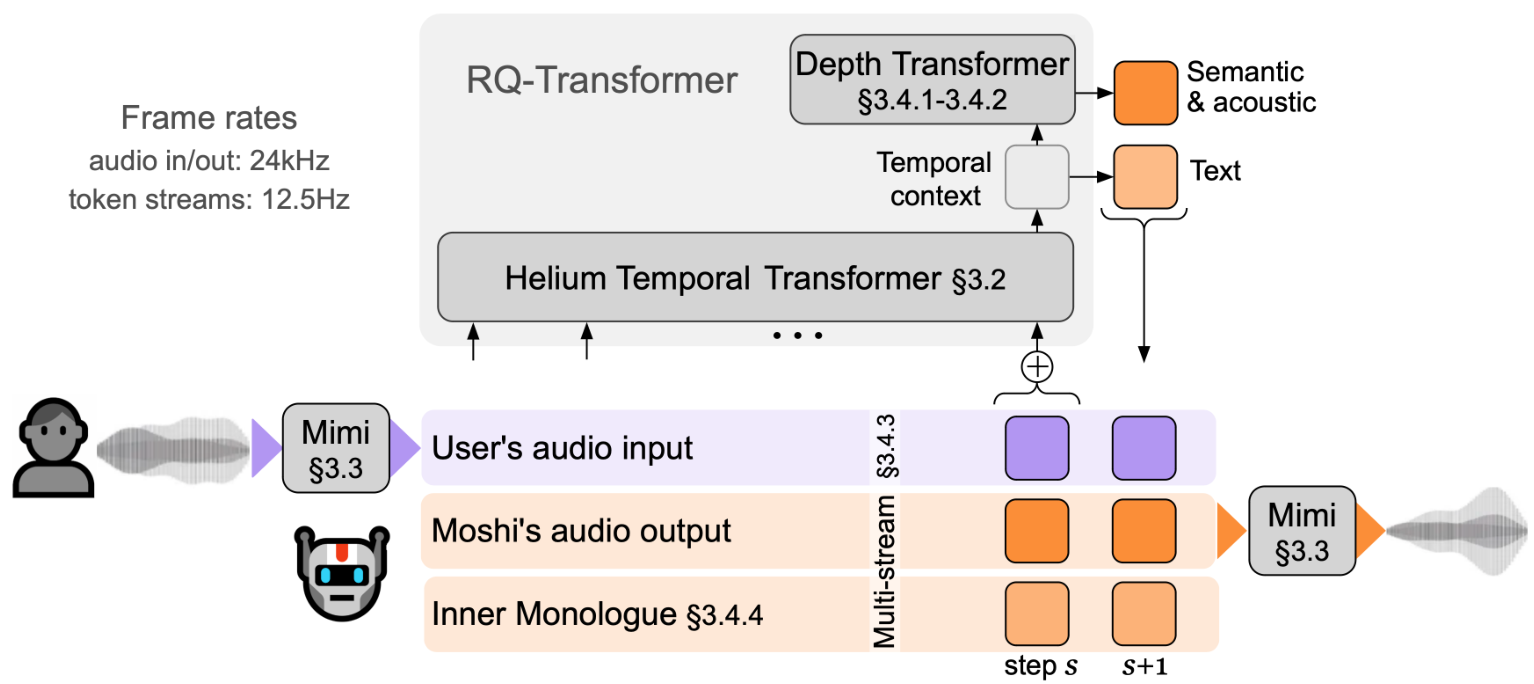
\includegraphics[width=\linewidth]{figures/papers/moshi.png}
\caption{\textbf{Moshi.} Reproduced from \citet{moshi}, Fig.~1. The temporal transformer coordinates user audio, assistant text and assistant audio; the depth transformer predicts acoustic codebooks. Think while listening adds silent reasoning and streaming ASR to the text stream \citep{thinklisten}; that extension is not shown in this source figure.}
\label{fig:detailed-moshi}
\end{figure}
\begin{figure}[H]
\centering
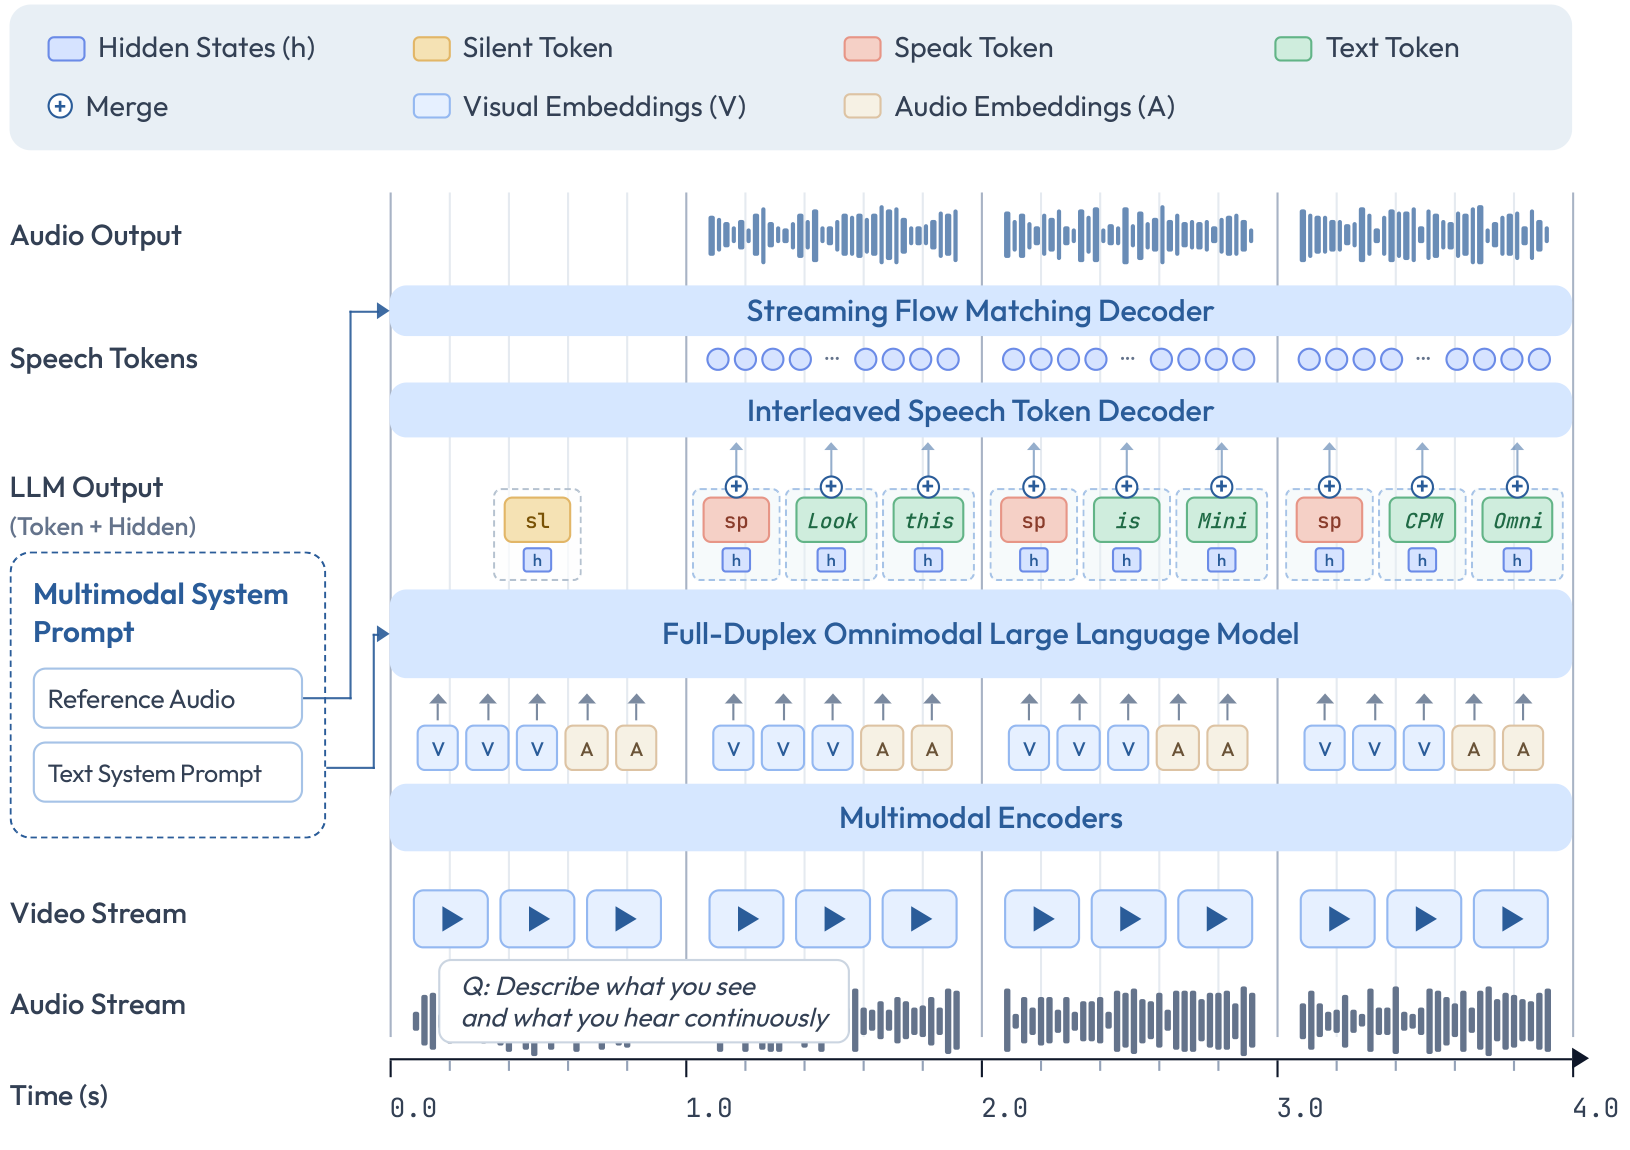
\includegraphics[width=0.94\linewidth]{figures/papers/minicpm.png}
\caption{\textbf{MiniCPM-o 4.5.} Reproduced from \citet{minicpm}, Fig.~4. A timed Qwen3-8B text backbone receives streaming multimodal input; separate speech-token and waveform decoders render its response. Open inference does not imply release of the complete training mixture.}
\label{fig:detailed-minicpm}
\end{figure}
\clearpage
\subsection{Original-paper architecture views: reasoning and delegation}
\begin{figure}[H]
\centering
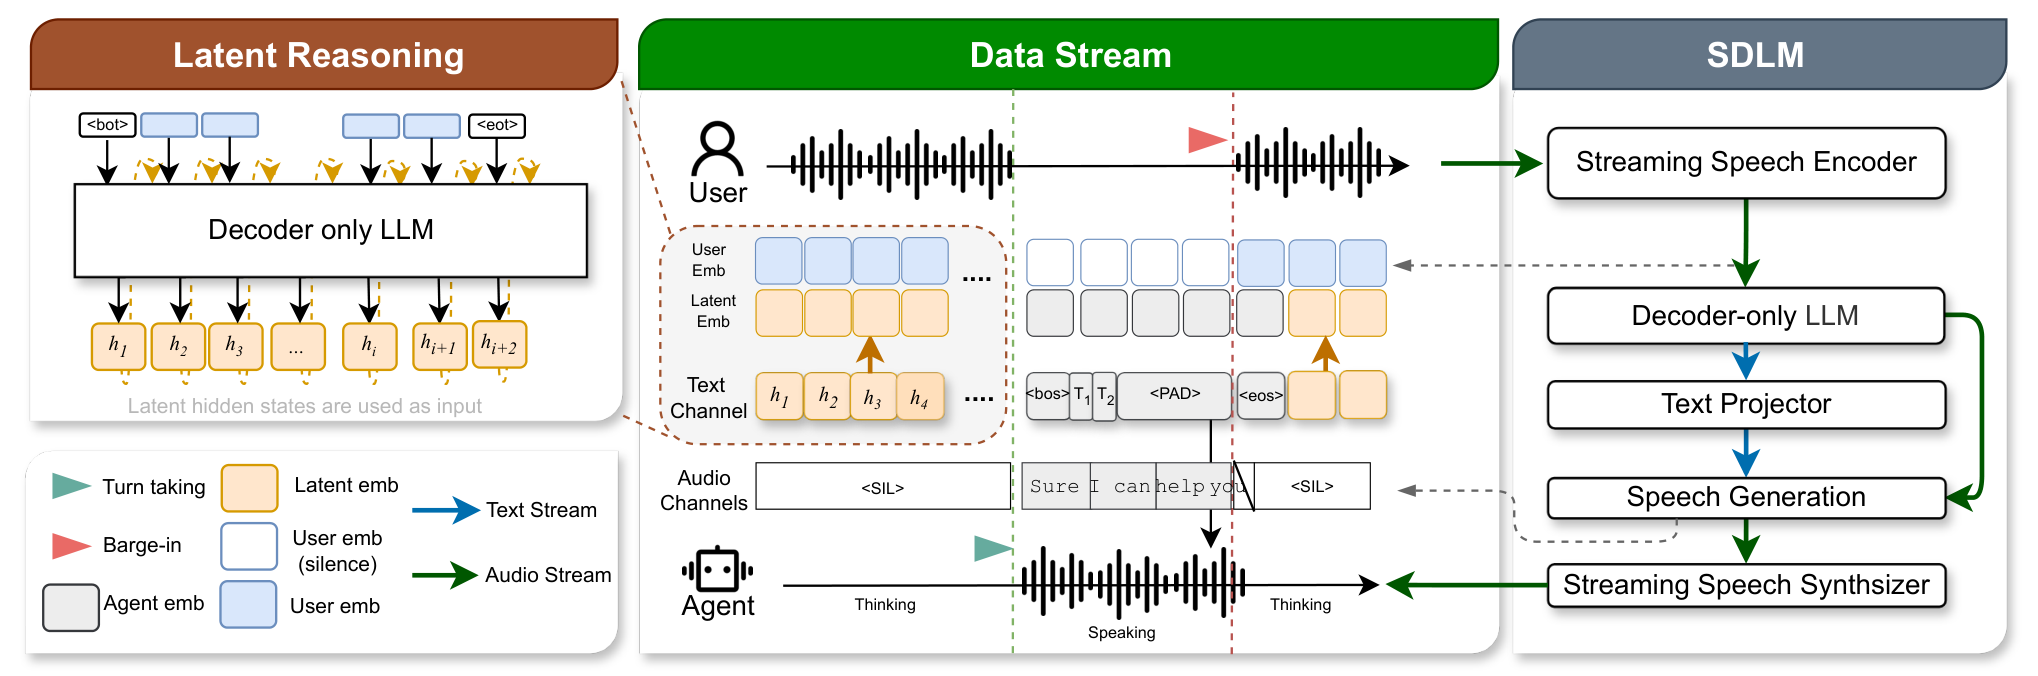
\includegraphics[width=0.96\linewidth]{figures/papers/flair.png}
\caption{\textbf{FLAIR.} Reproduced from \citet{flair}, Fig.~2. Latent reasoning while listening; text while speaking. The full-context expert is training-only.}
\label{fig:detailed-flair}
\end{figure}
\begin{figure}[H]
\centering
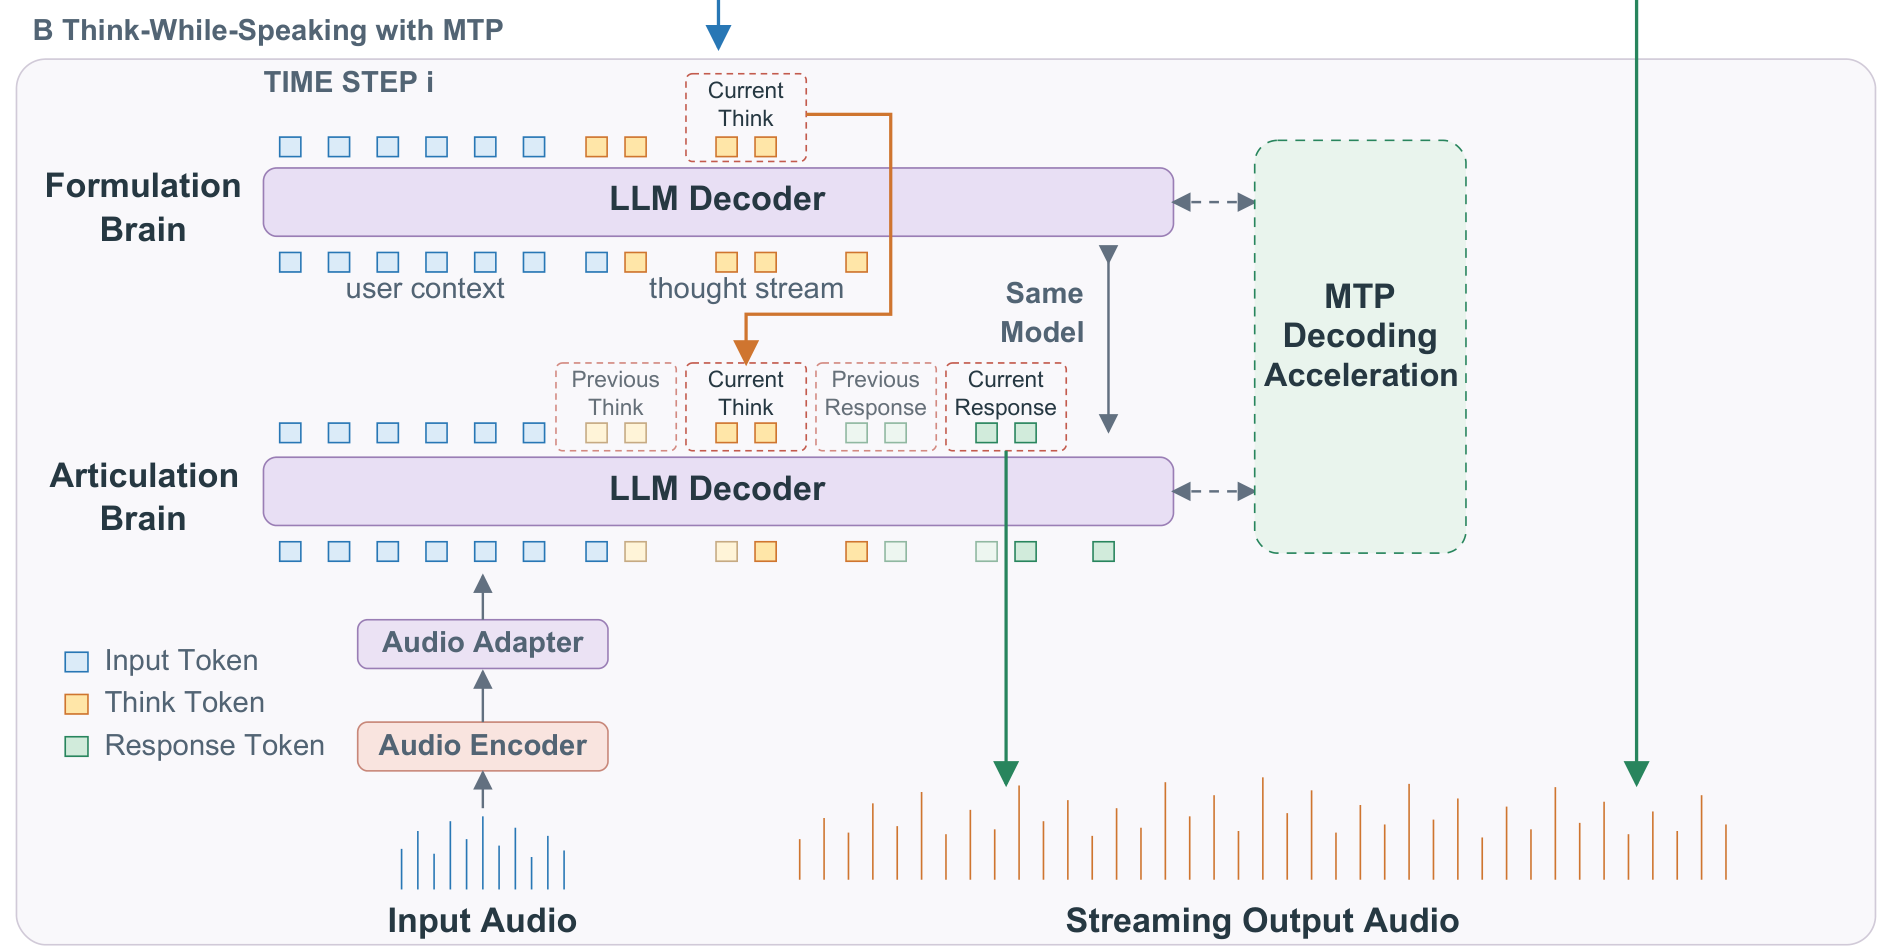
\includegraphics[width=0.78\linewidth]{figures/papers/step3.png}
\caption{\textbf{StepAudio 3 Realtime.} Reproduced from \citet{step3}, Fig.~7B (routing panel A omitted). Shared-model formulation/articulation; playback-aware pacing follows Mind-Paced Speaking \citep{mindpaced}.}
\label{fig:detailed-step3}
\end{figure}
\begin{figure}[H]
\centering
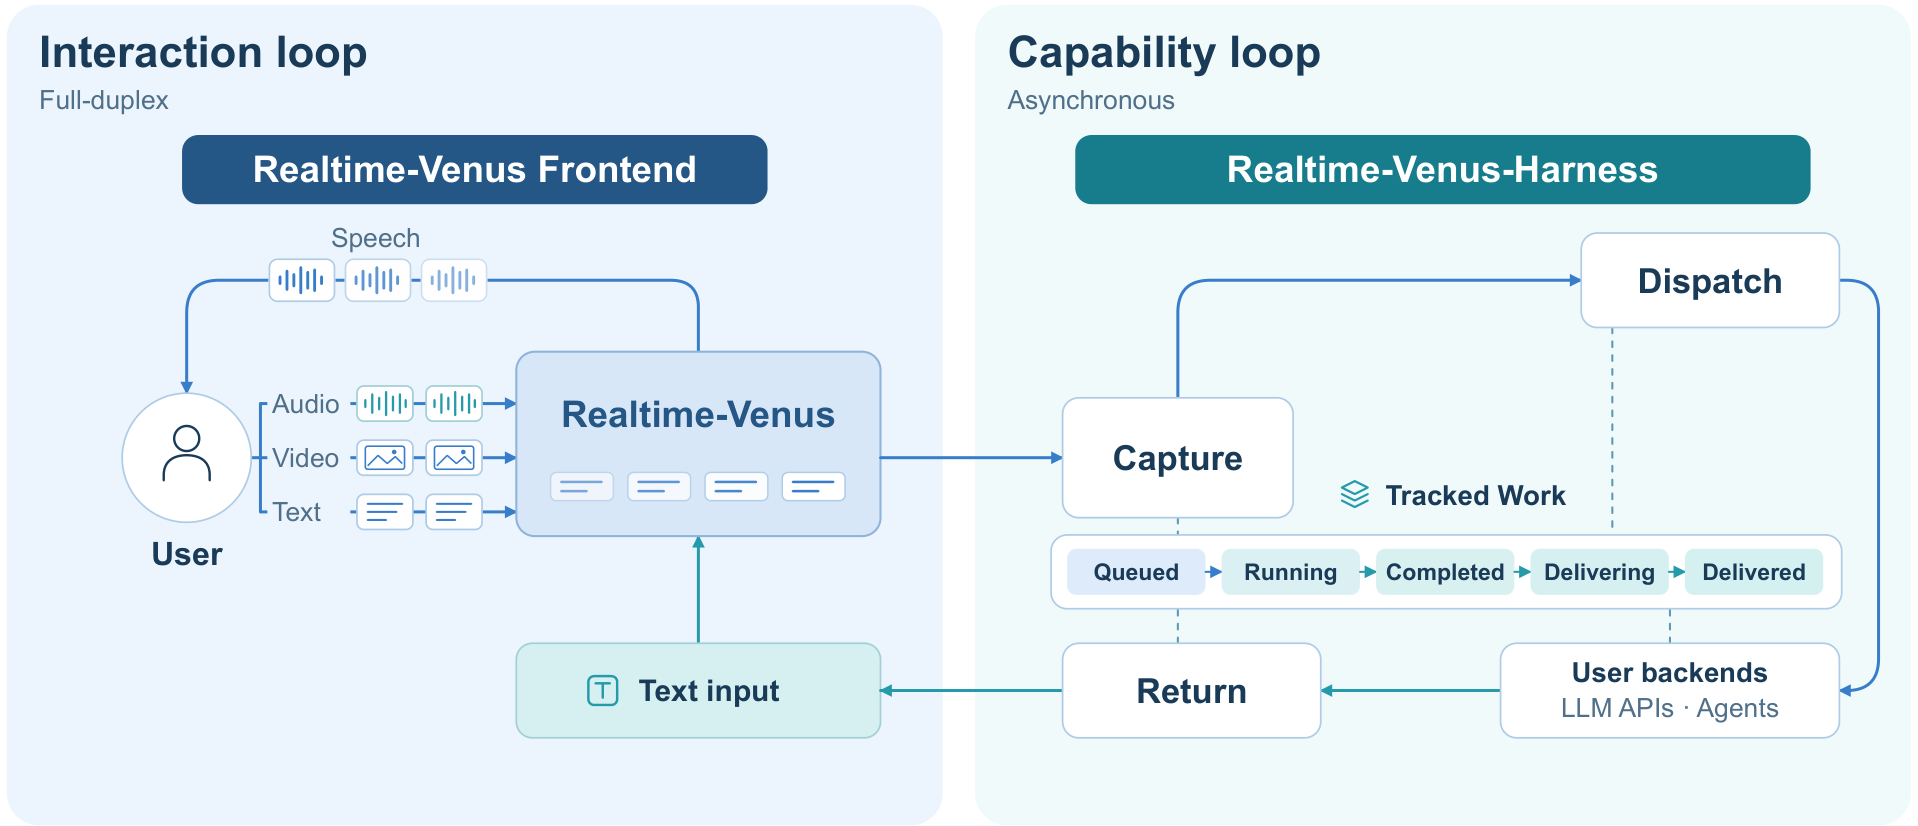
\includegraphics[width=0.95\linewidth]{figures/papers/venus.png}
\caption{\textbf{Realtime-Venus.} Reproduced from \citet{venus}, Fig.~3. Foreground interaction continues during delegation; the frontend controls reply-delivery timing.}
\label{fig:detailed-venus}
\end{figure}
\clearpage


\Needspace{12\baselineskip}
\subsection{Five synchronization and temporal-interface papers}
% Generated by scripts/generate.py; edit research/focused_review.py.
\begin{table}[H]
\centering
\small
\setlength{\tabcolsep}{4pt}
\setlength{\tablewidth}{\dimexpr\linewidth-6\tabcolsep\relax}
\renewcommand{\arraystretch}{1.12}
\caption{Synchronization and temporal interfaces. Five selected resources, unranked; availability checked 30 September 2026.}
\label{tab:synchronization}
\begin{tabular}{@{}>{\raggedright\arraybackslash}p{0.22\tablewidth}>{\raggedright\arraybackslash}p{0.30\tablewidth}>{\raggedright\arraybackslash}p{0.27\tablewidth}>{\raggedright\arraybackslash}p{0.21\tablewidth}@{}}
\toprule
\textbf{Paper} & \textbf{Temporal mechanism} & \textbf{What it establishes} & \textbf{Access / remaining issue} \\
\midrule
\textbf{SyncLLM}\par\citep{syncllm} & Llama 3-8B with deduplicated HuBERT units (25 Hz before deduplication); periodic speaker/chunk tokens align the sequence to a real-world clock. Speculative user chunks are replaced by observed input. & Synchronous full-duplex scheduling despite variable token counts; evaluates processing/network delay. & Official paper/demos; model code/weights not located. Clock alignment alone does not establish revision correctness.\par \href{https://syncllm.cs.washington.edu/}{Project}. \\
\addlinespace[4pt]
\textbf{Moshi}\par\citep{moshi} & Mimi 12.5 Hz (80 ms) frames; temporal transformer plus depth transformer model parallel audio streams and aligned inner-monologue text. & A concrete shared acoustic grid, streaming speech generation, and low-latency duplex interaction. & Inference and fine-tuning code + weights. MIT/Apache code; model CC BY 4.0. A frame clock is not a semantic commitment policy.\par \href{https://github.com/kyutai-labs/moshi}{Code}; \href{https://github.com/kyutai-labs/moshi-finetune}{Fine-tuning}; \href{https://huggingface.co/kyutai/moshiko-pytorch-bf16}{Weights}. \\
\addlinespace[4pt]
\textbf{DuplexSLA}\par\citep{duplexsla} & Step-Audio 2 mini-derived \textasciitilde{}7B model. A 160 ms clock joins two 80 ms listening features, one text/four audio tokens, and up to ten action tokens; queued action spillover and dual-side ASR. & Native concurrent speaking/listening plus timestamp-aligned planning, control and tool events. & Official repository says inference, weights and benchmark are forthcoming. Not a released checkpoint as of cutoff.\par \href{https://github.com/hyzhang24/DuplexSLA}{Release status}. \\
\addlinespace[4pt]
\textbf{AdaptDuplex}\par\citep{adapt} & Qwen3-Omni Thinker/Talker; 0.48/0.64/0.96 s windows, bounded text lead, and up to four indexed backend jobs. Cancelled/stale results are suppressed before injection. & Adaptive granularity and explicit backend-result admission already exist; not a new idea to simply cancel a stale job. & Paper verified; dedicated code/checkpoint not located. Joint speaker-owned state and actual playback still need controlled tests. \\
\addlinespace[4pt]
\textbf{Synchronization and Turn-Taking}\par\citep{synchrony} & Moshi--Moshi appointment dialogues: lagged CKA compares speaker/listener hidden states; causal probes classify end-of-interpausal-unit hold/non-hold events. & Representational coupling and predictive timing signals vary with noise and speech activity bias. & Preprint; study artifacts not located. Restricted task; CKA/probe success is not causal reasoning consistency. \\
\bottomrule
\end{tabular}
\end{table}

Table~\ref{tab:synchronization} separates \emph{acoustic synchronization}, \emph{compute scheduling}, \emph{action/event alignment}, and \emph{representation-level coupling}. A shared 80 or 160 ms grid can align streams without deciding whether a task hypothesis is ready to be spoken. Conversely, a good semantic answer can still miss its real-time deadline or be based on stale input. The Moshi--Moshi synchronization study provides evidence about hidden-state coupling and turn-taking signals, not a guarantee of correct state revision \citep{synchrony}.

The newest designs weaken several easy novelty claims. DuplexSLA already aligns speaking, listening and structured actions on one clock; its repository nevertheless marks inference, checkpoints and the benchmark as forthcoming \citep{duplexsla}. AdaptDuplex already supports variable windows, bounded text lead, indexed job cancellation and suppression of stale results \citep{adapt}. A project on synchronization must therefore test a stronger property---such as consistency between speaker-owned evidence, returned results and actual audible commitments---rather than claim that adaptation or cancellation itself is missing.

DuplexOmni supplies another explicit stop/reset mechanism for background thinking, while VoiceChat exposes a concrete blind interval during tool execution \citep{duplexomni,voicechat}. Neither background concurrency nor a native function head establishes that newly spoken corrections are incorporated before a returned result reaches the listener.

\Needspace{12\baselineskip}
\subsection{Five evaluation resources}
% Generated by scripts/generate.py; edit research/focused_review.py.
\begin{table}[H]
\centering
\small
\setlength{\tabcolsep}{4pt}
\setlength{\tablewidth}{\dimexpr\linewidth-6\tabcolsep\relax}
\renewcommand{\arraystretch}{1.12}
\caption{Benchmarks for the proposal. Five selected resources, unranked; availability checked 30 September 2026.}
\label{tab:benchmarks}
\begin{tabular}{@{}>{\raggedright\arraybackslash}p{0.22\tablewidth}>{\raggedright\arraybackslash}p{0.28\tablewidth}>{\raggedright\arraybackslash}p{0.25\tablewidth}>{\raggedright\arraybackslash}p{0.25\tablewidth}@{}}
\toprule
\textbf{Benchmark} & \textbf{Coverage / provenance} & \textbf{Useful measurements} & \textbf{Availability / blind spot} \\
\midrule
\textbf{SRQA}\par\citep{thinklisten} & TTS/LLM-rewritten ARC-E/C, SIQA, PIQA, GSM8K; mostly single-turn synthetic spoken questions. & Reasoning accuracy and post-question chain-of-thought delay; prefix sufficiency controls. & Construction in ICLR paper; released audio/eval package not located. CoT onset is not first useful audible answer. \\
\addlinespace[4pt]
\textbf{$\tau$-Voice}\par\citep{tauvoice} & 278 airline/retail/telecom tasks; clean/realistic speech; full-duplex simulated user. ICML 2026 (PMLR 306). & Grounded pass@1, interruption behavior and voice interaction quality; tool/task consequences. & Code/tasks/simulator; provider APIs needed. Virtual time decouples simulation from wall-clock runtime; pin original revision (repo now tau3-bench).\par \href{https://github.com/sierra-research/tau2-bench}{Code/tasks}. \\
\addlinespace[4pt]
\textbf{Full-Duplex-Bench v3}\par\citep{fdb3} & Human recordings, five disfluency types, chained tools across four task domains. & Tool-selection F1, argument accuracy, pass@1; first response, tool and completion latencies. & Scoring/inference code + recording download. Tool F1 is not task success; exact and judge-assisted argument scores differ.\par \href{https://github.com/DanielLin94144/Full-Duplex-Bench/tree/main/v3}{Code/data}. \\
\addlinespace[4pt]
\textbf{EchoChain}\par\citep{echochain} & 200 controlled interrupted conversations; synthesized user/barge-in audio; four closed realtime models; paired half-duplex control. & Conversation/criterion pass rates and failures: contextual inertia, interruption amnesia, objective displacement. & Paper, prompts and examples verified; standalone code/audio release not located. Does not cover backchannels, side speech or detailed acoustic timing. \\
\addlinespace[4pt]
\textbf{Duplex-MPE}\par\citep{mpe} & 2,000 matched pairs / 4,000 synthetic streams; 3--4 human roles plus assistant; explicit/implicit address. & Response initiation, answer accuracy, silence preservation, floor release; speaker-owned update controls. & Paper verified; standalone code/audio release not located. Floor release is conditional on the assistant already speaking. \\
\bottomrule
\end{tabular}
\end{table}

Table~\ref{tab:benchmarks} covers complementary failure modes. SRQA is suitable for early reasoning onset; $\tau$-Voice for grounded outcomes; Full-Duplex-Bench v3 for natural disfluency and tools; EchoChain for mid-generation task-state revision; and Duplex-MPE for silence/addressee control. $\tau$-Voice now has an ICML 2026 publisher record, updating its earlier preprint label \citep{tauvoice}. Its virtual-time simulator deliberately decouples simulated conversation from physical inference time. Task success there is valuable but cannot, by itself, validate wall-clock scheduling under contention.

EchoChain is especially close to the proposal: it diagnoses a failure to apply a correction, loss of earlier constraints, and abandonment of the original goal after interruption \citep{echochain}. We should reuse this conceptual distinction rather than present correction-sensitive reasoning as unevaluated. Its fixed speech-onset-relative injection and closed-model evaluation leave useful extensions: instrument the input evidence actually incorporated, distinguish generated from played audio, and include irrelevant or other-directed speech. The five benchmark scores measure different conditions and should not be averaged or interpreted as a common leaderboard.

\Needspace{12\baselineskip}
\subsection{Five conversational training and supervision resources}
% Generated by scripts/generate.py; edit research/focused_review.py.
\begin{table}[H]
\centering
\small
\setlength{\tabcolsep}{4pt}
\setlength{\tablewidth}{\dimexpr\linewidth-6\tabcolsep\relax}
\renewcommand{\arraystretch}{1.12}
\caption{Training data and supervision sources. Five selected resources, unranked; availability checked 30 September 2026.}
\label{tab:data}
\begin{tabular}{@{}>{\raggedright\arraybackslash}p{0.20\tablewidth}>{\raggedright\arraybackslash}p{0.22\tablewidth}>{\raggedright\arraybackslash}p{0.28\tablewidth}>{\raggedright\arraybackslash}p{0.30\tablewidth}@{}}
\toprule
\textbf{Resource} & \textbf{Scale / channels} & \textbf{What is annotated} & \textbf{Access / project use} \\
\midrule
\textbf{SmoothConv}\par\citep{smoothconv} & 100.53 h; Chinese; natural multi-party, multi-channel audio. & Expert transcripts, speaker IDs, turn state, timing and paralinguistic labels. & HF release; CC BY-NC 4.0. Control/speaker supervision; shares source conversations with DuplexConv.\par \href{https://huggingface.co/datasets/qualialabsAI/SmoothConv}{Dataset card}. \\
\addlinespace[4pt]
\textbf{DuplexConv}\par\citep{duplexconv} & 2,000.21 h; Chinese; natural multi-party, multi-channel audio. & LLM-assisted transcripts, per-track VAD, speaker/turn segments, acoustic and scene labels. & HF release; CC BY-NC 4.0. Larger timing pretraining; audit labels and split by underlying source session.\par \href{https://huggingface.co/datasets/OpenT2S/DuplexConv}{Dataset card}. \\
\addlinespace[4pt]
\textbf{otoSpeech Task}\par\citep{ototask} & 20.006 h; 58 English sessions; two-speaker 48 kHz channels; seven task types. & Synchronized events, stimuli, participant artifacts and task-related metadata. & Gated HF files/contact acceptance; CC BY 4.0. Task-evidence alignment; verify outcomes before treating as reasoning labels.\par \href{https://huggingface.co/datasets/otoearth/otoSpeech-full-duplex-task-oriented-20h}{Dataset card}. \\
\addlinespace[4pt]
\textbf{otoSpeech conversational}\par\citep{otoconv} & 280 h raw / 141 h curated; English; separate speaker channels; curated 44.1 kHz. & Session/speaker metadata, redactions, surveys; natural overlap and timing. & Gated HF files/contact acceptance; CC BY 4.0. Listening robustness; curated hours are a subset, not extra data.\par \href{https://huggingface.co/datasets/otoearth/otoSpeech-full-duplex-processed-141h}{Dataset card}. \\
\addlinespace[4pt]
\textbf{Open Yap 1K}\par\citep{openyap} & 1,000 h; 1,602 English conversations; 239 speakers; separate 48 kHz channels. & Word-level transcripts, speaker/device metadata, overlap and turn-gap statistics. & Public sample; full corpus by request/Data Use Agreement. Natural conversation, not an ungated full release.\par \href{https://github.com/The-Agentic-Data-Co/open-yap-1k}{Release/terms}. \\
\bottomrule
\end{tabular}
\end{table}

The five resources in Table~\ref{tab:data} supply natural timing, channels, speaker identity or task events. None automatically supplies a label saying ``this prefix supports this reasoning step'' or ``this correction invalidates that claim.'' SmoothConv and DuplexConv share underlying conversational sources: split by original session \emph{before} using one for training and the other for evaluation. The curated otoSpeech hours are a subset of its raw hours; Open Yap's sample is not its full corpus. Non-commercial restrictions, gated access and Data Use Agreements constrain any eventual release or usage.

A small supervision layer should identify the evidence interval for a claim, earliest causally sufficient prefix, source speaker/addressee, task-state revision, and whether the affected output has already been played. Use counterfactual suffixes with an identical prefix to detect premature conclusions, and retain negative examples with backchannels and side speech. The reported spoken-CoT construction in Think while listening is a useful recipe, not an independently released 1.8M-example dataset \citep{thinklisten}. Use held-out benchmark tests for evaluation, not as an unreported source of training supervision.

\clearpage
\section{Reported benchmark performance and model profiles}
\label{sec:performance}
% Generated by scripts/build_performance.py; edit the structured sources.
\subsection{What is reported, and what is missing}
The five selected systems have sparse coverage across the selected benchmark families (Figure~\ref{fig:performance-coverage}). Missing results are NR, not zero. FLAIR's separate study evaluations below do not fill an FDB-v3 or SRQA cell. Source versions, table/page locators and PDF hashes are archived alongside the reported values; these checks verify transcription, not experimental reproduction.
\begin{figure}[H]
\centering
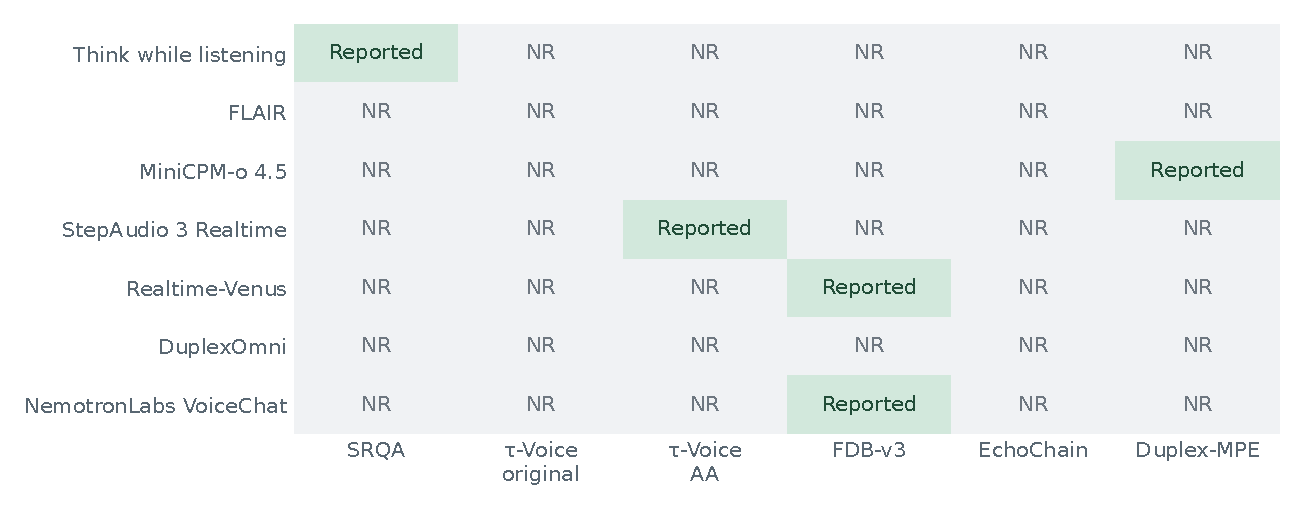
\includegraphics[width=\linewidth]{figures/performance/coverage.pdf}
\caption{Reported selected-system coverage in the five benchmark families, with the two $\tau$-Voice implementations kept separate. NR means no matching result was located in the reviewed sources.}
\label{fig:performance-coverage}
\end{figure}
\paragraph{How to read the profiles.}
Radars show raw percentages on a shared 0--100 scale within one protocol; their area is not a model score. Separate bars are used for mixed units or fewer than three metrics. Solid lines denote selected configurations; dashed lines denote reference/ablation configurations. Compare named curves and individual metrics, not polygon area or panels from different benchmarks. No missing cell is imputed and no cross-benchmark average is calculated. The figures use source-reported point estimates, without reproducing experiments or inventing uncertainty bars.
Closed references are benchmark-source leaders where reported, not current global SoTA. SRQA and Duplex-MPE do not test a closed voice system. FLAIR's historical interaction table contains only one closed API reference, with no precise revision. Imported reference scores and later system-report evaluations are not a common rerun.
\clearpage
\subsection{Think while listening: SRQA}
Two TWL-study checkpoints are distinct. Kimi-Audio is a speech reference, not a full-duplex system. The table also includes Qwen2-Audio; Helium's non-comparable text result is omitted. \citep{thinklisten}
\begin{figure}[H]
\centering
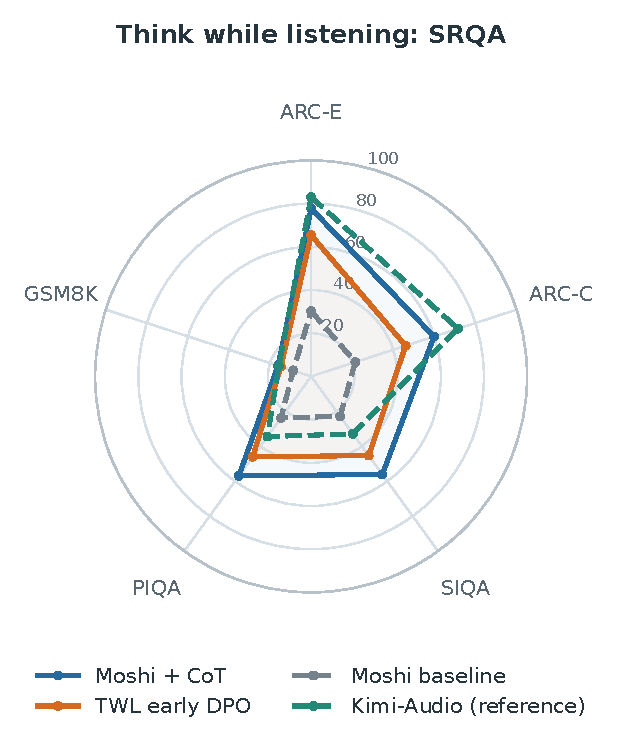
\includegraphics[width=0.78\linewidth]{figures/performance/twl.pdf}
\caption{Think while listening: SRQA. Raw percentages; higher is better. Exact values and additional context references are in the adjacent table.}
\label{fig:performance-twl}
\end{figure}
% Generated by scripts/build_performance.py; edit research/reported-performance.json.
\begin{table}[H]
\centering\small
\setlength{\tabcolsep}{3pt}
\setlength{\tablewidth}{\dimexpr\linewidth-10\tabcolsep\relax}
\renewcommand{\arraystretch}{1.06}
\caption{SRQA. Percent; higher is better. Bold: best among the displayed references, not a source-wide or current SoTA. \citep{thinklisten}}
\label{tab:performance-srqa}
\begin{tabular}{@{}>{\raggedright\arraybackslash}p{0.32\tablewidth}>{\centering\arraybackslash}p{0.136000\tablewidth}>{\centering\arraybackslash}p{0.136000\tablewidth}>{\centering\arraybackslash}p{0.136000\tablewidth}>{\centering\arraybackslash}p{0.136000\tablewidth}>{\centering\arraybackslash}p{0.136000\tablewidth}@{}}
\toprule
\textbf{Model / configuration} & \textbf{ARC-E} & \textbf{ARC-C} & \textbf{SIQA} & \textbf{PIQA} & \textbf{GSM8K} \\
\midrule
\textbf{Moshi + CoT (TWL study)} & 77.7 & 59.8 & \textbf{56.1} & \textbf{56.9} & 16.1 \\
\textbf{TWL: early length-DPO} & 65.4 & 46.0 & 45.3 & 46.0 & 14.7 \\
Moshi baseline & 30.2 & 21.5 & 22.8 & 23.8 & 8.7 \\
Kimi-Audio-7B-Instruct & \textbf{83.0} & \textbf{71.5} & 32.9 & 34.4 & 15.7 \\
Qwen2-Audio-7B-Instruct & 59.1 & 42.4 & 21.9 & 24.5 & \textbf{18.1} \\
\bottomrule
\end{tabular}
\end{table}

{\small\textbf{Reading this profile (review interpretation).} The CoT configuration is stronger on these tasks than foundation Moshi, but early length-DPO is a different accuracy/latency operating point, not the same high-accuracy checkpoint.}
\clearpage
\subsection{FLAIR: spoken QA accuracy}
FLAIR's own QA suite is not SRQA. Only accuracy-valued tasks are plotted; 1–5 open-ended judge scores are excluded. Published reference scores are imported, not all rerun. Kimi-Audio is half-duplex. \citep{flair}
\begin{figure}[H]
\centering
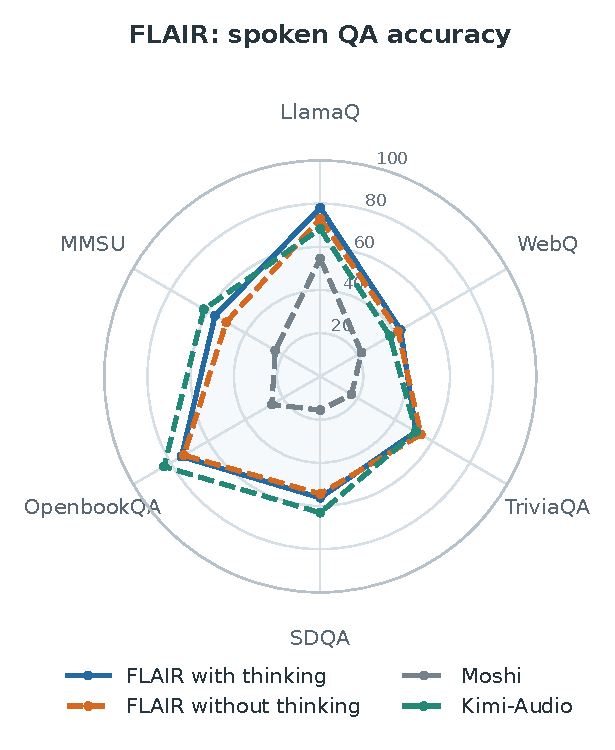
\includegraphics[width=0.78\linewidth]{figures/performance/flair-qa.pdf}
\caption{FLAIR: spoken QA accuracy. Raw percentages; higher is better. Exact values and additional context references are in the adjacent table.}
\label{fig:performance-flair-qa}
\end{figure}
% Generated by scripts/build_performance.py; edit research/reported-performance.json.
\begin{table}[H]
\centering\small
\setlength{\tabcolsep}{3pt}
\setlength{\tablewidth}{\dimexpr\linewidth-12\tabcolsep\relax}
\renewcommand{\arraystretch}{1.06}
\caption{FLAIR study: spoken QA. Percent; higher is better. Bold: best among the displayed references, not a source-wide or current SoTA. \citep{flair}}
\label{tab:performance-flair_qa}
\begin{tabular}{@{}>{\raggedright\arraybackslash}p{0.32\tablewidth}>{\centering\arraybackslash}p{0.113333\tablewidth}>{\centering\arraybackslash}p{0.113333\tablewidth}>{\centering\arraybackslash}p{0.113333\tablewidth}>{\centering\arraybackslash}p{0.113333\tablewidth}>{\centering\arraybackslash}p{0.113333\tablewidth}>{\centering\arraybackslash}p{0.113333\tablewidth}@{}}
\toprule
\textbf{Model / configuration} & \textbf{LlamaQ} & \textbf{WebQ} & \textbf{TriQA} & \textbf{SDQA} & \textbf{OBQA} & \textbf{MMSU} \\
\midrule
\textbf{FLAIR w/ thk} & \textbf{78.0} & \textbf{43.0} & 51.2 & 56.2 & 74.2 & 56.2 \\
FLAIR w/o thk & 73.0 & 41.7 & \textbf{53.8} & 54.4 & 72.9 & 50.2 \\
Moshi & 54.5 & 22.1 & 16.7 & 15.6 & 25.9 & 24.0 \\
Freeze-Omni & 56.2 & 27.9 & 28.5 & 53.5 & 31.0 & 28.1 \\
Kimi-Audio & 68.3 & 37.3 & 51.2 & \textbf{63.1} & \textbf{83.5} & \textbf{62.2} \\
\bottomrule
\end{tabular}
\end{table}

{\small\textbf{Reading this profile (review interpretation).} Latent thinking improves several tasks over the no-thinking ablation, but not every task: TriviaQA is lower. No single curve wins across all tasks shown.}
\clearpage
\subsection{FLAIR: earlier duplex interaction suite}
Separate axes preserve percentages, seconds and 0–5 judge scores. TOR means takeover rate. Gemini Live is the study's sole closed reference; its API revision is unspecified. This is not FDB-v3 tool use. \citep{flair}
\begin{figure}[H]
\centering
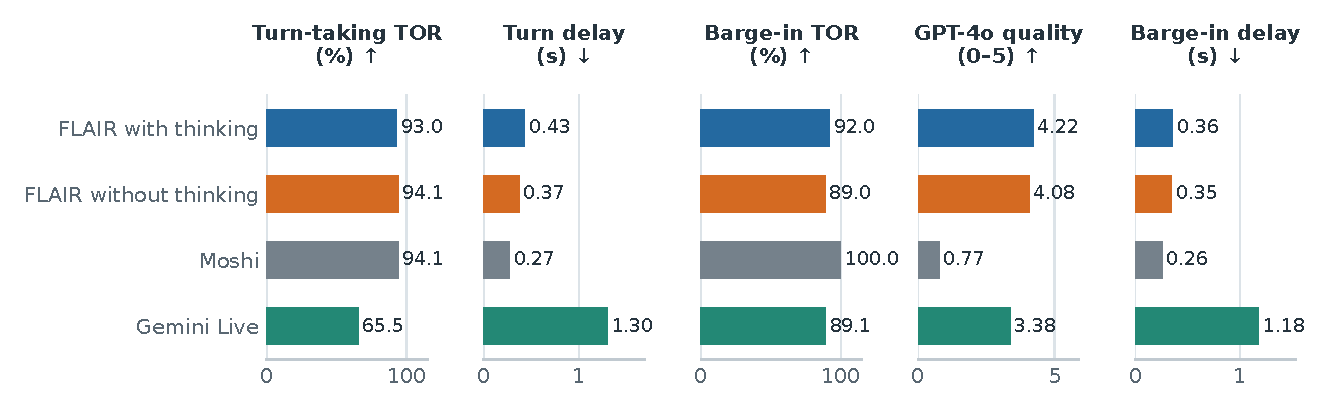
\includegraphics[width=\linewidth]{figures/performance/flair-interaction.pdf}
\caption{FLAIR: earlier duplex interaction suite. Units and directions are labeled per panel. Exact values and additional context references are in the adjacent table.}
\label{fig:performance-flair-interaction}
\end{figure}
% Generated by scripts/build_performance.py; edit research/reported-performance.json.
\begin{table}[H]
\centering\small
\setlength{\tabcolsep}{3pt}
\setlength{\tablewidth}{\dimexpr\linewidth-10\tabcolsep\relax}
\renewcommand{\arraystretch}{1.06}
\caption{FLAIR study: Full-Duplex-Bench (original suite). Each column states its unit and direction. Bold: best among the displayed references, not a source-wide or current SoTA. \citep{flair}}
\label{tab:performance-flair_interaction}
\begin{tabular}{@{}>{\raggedright\arraybackslash}p{0.32\tablewidth}>{\centering\arraybackslash}p{0.136000\tablewidth}>{\centering\arraybackslash}p{0.136000\tablewidth}>{\centering\arraybackslash}p{0.136000\tablewidth}>{\centering\arraybackslash}p{0.136000\tablewidth}>{\centering\arraybackslash}p{0.136000\tablewidth}@{}}
\toprule
\textbf{Model / configuration} & \textbf{Turn-taking TOR (\%; higher)} & \textbf{Turn-taking latency (s; lower)} & \textbf{Barge-in TOR (\%; higher)} & \textbf{Barge-in GPT-4o (0–5; higher)} & \textbf{Barge-in latency (s; lower)} \\
\midrule
\textbf{FLAIR w/ thk} & 93.0 & 0.43 & 92.0 & \textbf{4.22} & 0.36 \\
FLAIR w/o thk & \textbf{94.1} & 0.37 & 89.0 & 4.08 & 0.35 \\
Moshi & \textbf{94.1} & \textbf{0.27} & \textbf{100.0} & 0.77 & \textbf{0.26} \\
Gemini Live & 65.5 & 1.30 & 89.1 & 3.38 & 1.18 \\
\bottomrule
\end{tabular}
\end{table}

{\small\textbf{Reading this profile (review interpretation).} Response quality, takeover rate and response delay expose different trade-offs. A high takeover rate alone does not establish a useful answer.}
\clearpage
\subsection{StepAudio 3 Realtime: $\tau$-Voice (AA)}
Artificial Analysis implementation and API versions from StepAudio's report. The radar shows three domain success rates; the bar panel shows the separately reported equal-domain macro. Grok is the macro leader, not the winner in every domain. \citep{step3}
\begin{figure}[H]
\centering
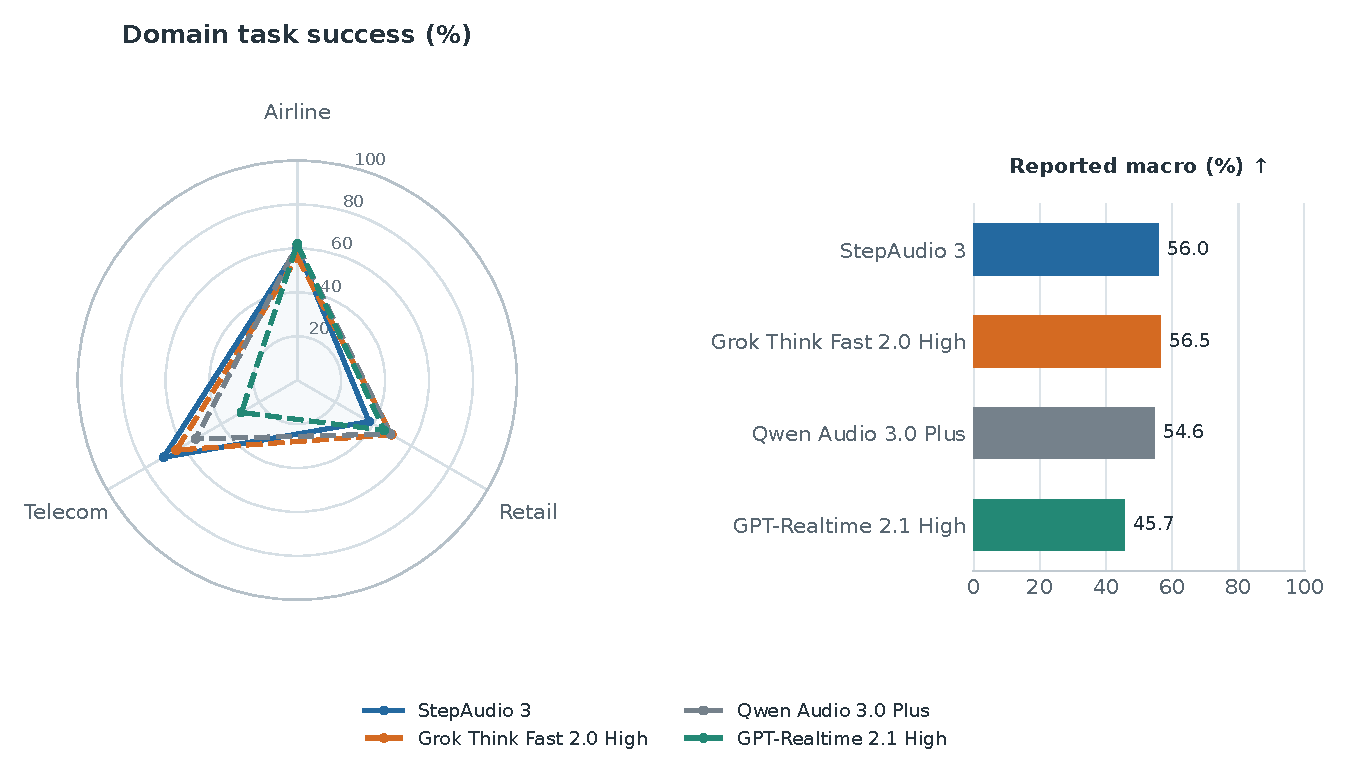
\includegraphics[width=\linewidth]{figures/performance/step3.pdf}
\caption{StepAudio 3 Realtime: $\tau$-Voice (AA). Raw percentages; higher is better. Exact values and additional context references are in the adjacent table.}
\label{fig:performance-step3}
\end{figure}
% Generated by scripts/build_performance.py; edit research/reported-performance.json.
\begin{table}[H]
\centering\small
\setlength{\tabcolsep}{3pt}
\setlength{\tablewidth}{\dimexpr\linewidth-8\tabcolsep\relax}
\renewcommand{\arraystretch}{1.06}
\caption{$\tau$-Voice (AA). Percent; higher is better. Bold: best among the displayed references, not a source-wide or current SoTA. \citep{step3}}
\label{tab:performance-tau_aa}
\begin{tabular}{@{}>{\raggedright\arraybackslash}p{0.32\tablewidth}>{\centering\arraybackslash}p{0.170000\tablewidth}>{\centering\arraybackslash}p{0.170000\tablewidth}>{\centering\arraybackslash}p{0.170000\tablewidth}>{\centering\arraybackslash}p{0.170000\tablewidth}@{}}
\toprule
\textbf{Model / configuration} & \textbf{Airline} & \textbf{Retail} & \textbf{Telecom} & \textbf{Macro task success} \\
\midrule
\textbf{StepAudio 3 Realtime} & 60.0 & 37.7 & \textbf{70.2} & 56.0 \\
Grok Voice Think Fast 2.0 High & 56.0 & \textbf{49.7} & 63.7 & \textbf{56.5} \\
Qwen Audio 3.0 Realtime Plus & 61.3 & 49.0 & 53.5 & 54.6 \\
GPT-Realtime-2.1 High & \textbf{62.0} & 45.6 & 29.4 & 45.7 \\
\bottomrule
\end{tabular}
\end{table}

{\small\textbf{Reading this profile (review interpretation).} The reported macro scores are close while the domain profiles differ. This comparison cannot be pooled with the original clean/realistic $\tau$-Voice results.}
\clearpage
\subsection{Realtime-Venus: Full-Duplex-Bench v3}
Both Venus frontends are from the revised system report; closed references are from the benchmark comparison. GPT-Realtime leads these three metrics in that source, not a current global leaderboard. This is not a common rerun. \citep{fdb3,venus}
\begin{figure}[H]
\centering
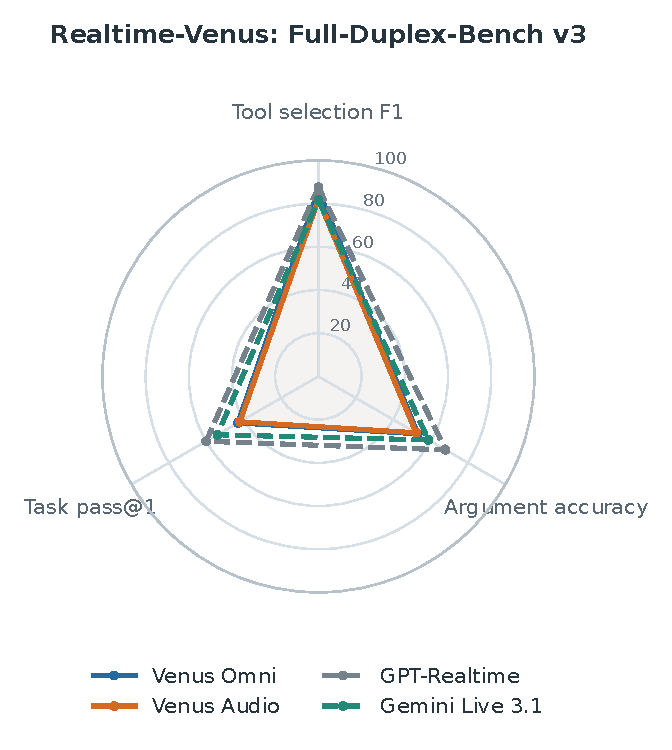
\includegraphics[width=0.78\linewidth]{figures/performance/venus.pdf}
\caption{Realtime-Venus: Full-Duplex-Bench v3. Raw percentages; higher is better. Exact values and additional context references are in the adjacent table.}
\label{fig:performance-venus}
\end{figure}
% Generated by scripts/build_performance.py; edit research/reported-performance.json.
\begin{table}[H]
\centering\small
\setlength{\tabcolsep}{3pt}
\setlength{\tablewidth}{\dimexpr\linewidth-6\tabcolsep\relax}
\renewcommand{\arraystretch}{1.06}
\caption{Full-Duplex-Bench v3. Percent; higher is better. Bold: best among the displayed references, not a source-wide or current SoTA. \citep{fdb3,venus}}
\label{tab:performance-fdb3}
\begin{tabular}{@{}>{\raggedright\arraybackslash}p{0.32\tablewidth}>{\centering\arraybackslash}p{0.226667\tablewidth}>{\centering\arraybackslash}p{0.226667\tablewidth}>{\centering\arraybackslash}p{0.226667\tablewidth}@{}}
\toprule
\textbf{Model / configuration} & \textbf{Tool F1} & \textbf{Argument accuracy} & \textbf{Pass@1} \\
\midrule
\textbf{Realtime-Venus-Omni} & 86.0 & 53.1 & 43.0 \\
\textbf{Realtime-Venus-Audio} & 82.0 & 52.2 & 42.0 \\
GPT-Realtime & \textbf{87.6} & \textbf{68.0} & \textbf{60.0} \\
Gemini Live 3.1 & 81.7 & 58.8 & 54.0 \\
\bottomrule
\end{tabular}
\end{table}

{\small\textbf{Reading this profile (review interpretation).} Tool-selection F1 is substantially higher than complete-task pass@1. These metrics have different success criteria, so their difference is not a stage-wise failure rate.}
\clearpage
\subsection{MiniCPM-o 4.5: Duplex-MPE}
Explicit and implicit addressing are separate panels. Moshi and Voila are representative speech references. Answer accuracy is conditional on fresh responses; yield uses model-specific eligible speaking events. Polygon area is not an overall score. Gemini's transcript control is excluded. \citep{mpe}
\begin{figure}[H]
\centering
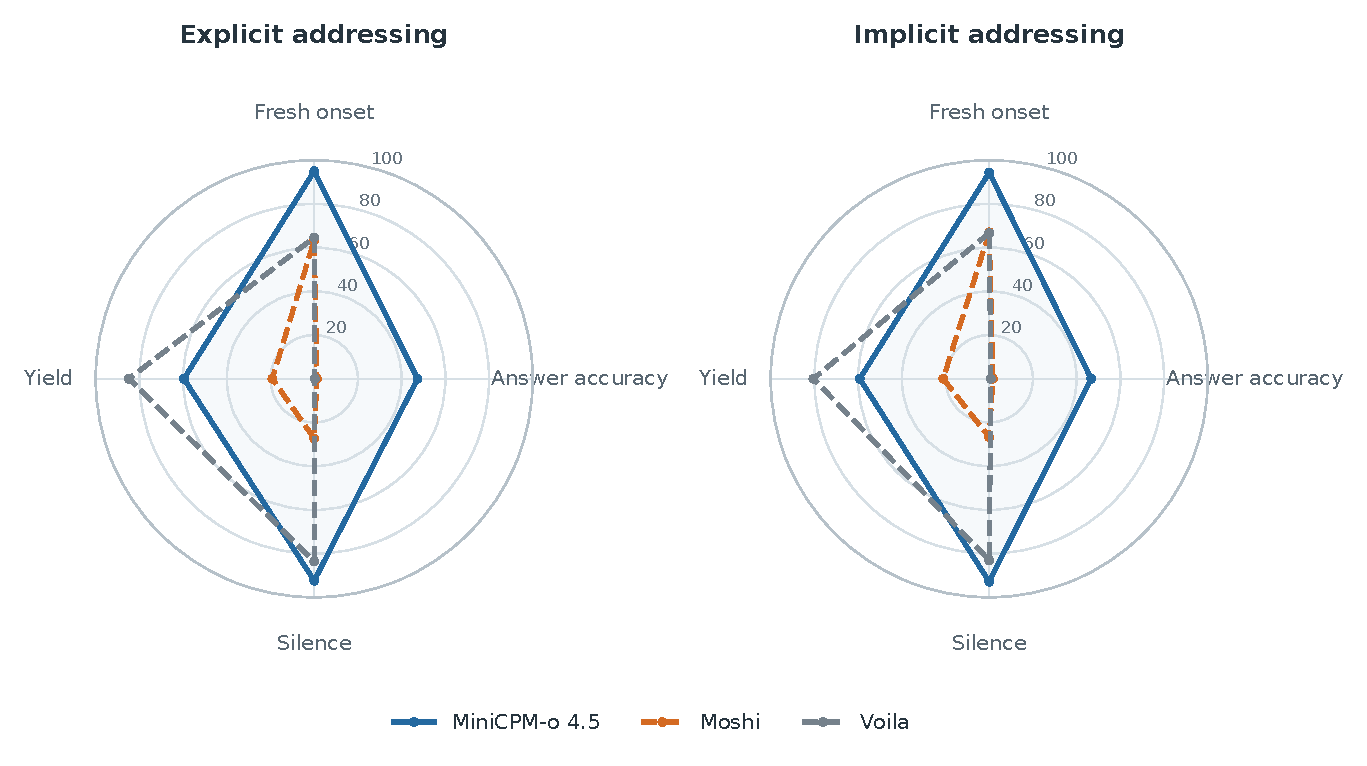
\includegraphics[width=\linewidth]{figures/performance/minicpm.pdf}
\caption{MiniCPM-o 4.5: Duplex-MPE. Raw percentages; higher is better. Exact values and additional context references are in the adjacent table.}
\label{fig:performance-minicpm}
\end{figure}
% Generated by scripts/build_performance.py; edit research/reported-performance.json.
\begin{table}[H]
\centering\small
\setlength{\tabcolsep}{3pt}
\setlength{\tablewidth}{\dimexpr\linewidth-8\tabcolsep\relax}
\renewcommand{\arraystretch}{1.06}
\caption{Duplex-MPE. Percent; higher is better. Bold: best among the displayed references, not a source-wide or current SoTA. \citep{mpe}}
\label{tab:performance-mpe}
\begin{tabular}{@{}>{\raggedright\arraybackslash}p{0.32\tablewidth}>{\centering\arraybackslash}p{0.170000\tablewidth}>{\centering\arraybackslash}p{0.170000\tablewidth}>{\centering\arraybackslash}p{0.170000\tablewidth}>{\centering\arraybackslash}p{0.170000\tablewidth}@{}}
\toprule
\textbf{Model / configuration} & \textbf{Fresh onset} & \textbf{Answer accuracy} & \textbf{Silence preservation} & \textbf{Yield} \\
\midrule
\textbf{MiniCPM-o 4.5 (explicit)} & \textbf{95.00} & \textbf{47.30} & 92.42 & 59.64 \\
\textbf{MiniCPM-o 4.5 (implicit)} & 94.35 & 46.65 & \textbf{92.89} & 59.25 \\
Voila (explicit) & 64.65 & 0.31 & 83.51 & \textbf{84.84} \\
Voila (implicit) & 66.70 & 0.75 & 83.07 & 80.46 \\
Moshi (explicit) & 63.40 & 1.23 & 27.34 & 19.18 \\
Moshi (implicit) & 67.00 & 1.70 & 26.76 & 21.07 \\
\bottomrule
\end{tabular}
\end{table}

{\small\textbf{Reading this profile (review interpretation).} MiniCPM-o combines frequent fresh responses and silence preservation, but conditional answer accuracy is much lower. Voila's higher yield is conditional on different eligible events.}
\clearpage
\subsection{Original $\tau$-Voice: closed voice references}
Original benchmark Table 6 All row; clean and realistic conditions remain separate. None of the five selected systems is evaluated here. GPT-5's text control is not plotted as a voice competitor. \citep{tauvoice}
\begin{figure}[H]
\centering
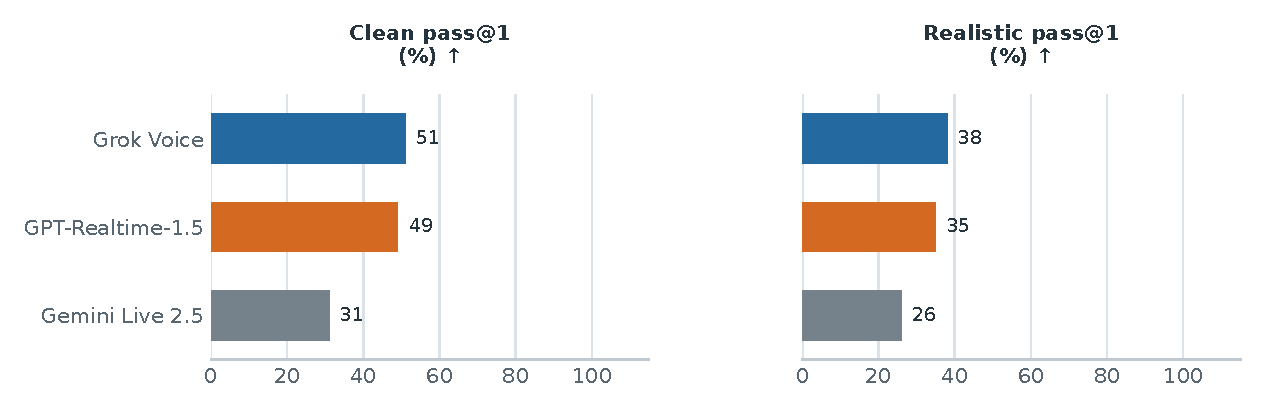
\includegraphics[width=\linewidth]{figures/performance/tau-original.pdf}
\caption{Original $\tau$-Voice: closed voice references. Units and directions are labeled per panel. Exact values and additional context references are in the adjacent table.}
\label{fig:performance-tau-original}
\end{figure}
% Generated by scripts/build_performance.py; edit research/reported-performance.json.
\begin{table}[H]
\centering\small
\setlength{\tabcolsep}{3pt}
\setlength{\tablewidth}{\dimexpr\linewidth-4\tabcolsep\relax}
\renewcommand{\arraystretch}{1.06}
\caption{$\tau$-Voice. Percent; higher is better. Bold: best among the displayed references, not a source-wide or current SoTA. \citep{tauvoice}}
\label{tab:performance-tau_original}
\begin{tabular}{@{}>{\raggedright\arraybackslash}p{0.32\tablewidth}>{\centering\arraybackslash}p{0.340000\tablewidth}>{\centering\arraybackslash}p{0.340000\tablewidth}@{}}
\toprule
\textbf{Model / configuration} & \textbf{Clean pass@1} & \textbf{Realistic pass@1} \\
\midrule
Grok Voice & \textbf{51} & \textbf{38} \\
GPT-Realtime-1.5 & 49 & 35 \\
Gemini Live 2.5 & 31 & 26 \\
\bottomrule
\end{tabular}
\end{table}

{\small\textbf{Reading this profile (review interpretation).} All three voice systems perform worse under realistic audio conditions in this source comparison; later $\tau$-Voice implementations are separate evidence.}
\clearpage
\subsection{EchoChain: closed voice references}
Paper Table 1, across 200 interrupted conversations. MPR requires every criterion in a conversation to pass; MCP scores individual criteria. None of the five selected systems is evaluated here. \citep{echochain}
\begin{figure}[H]
\centering
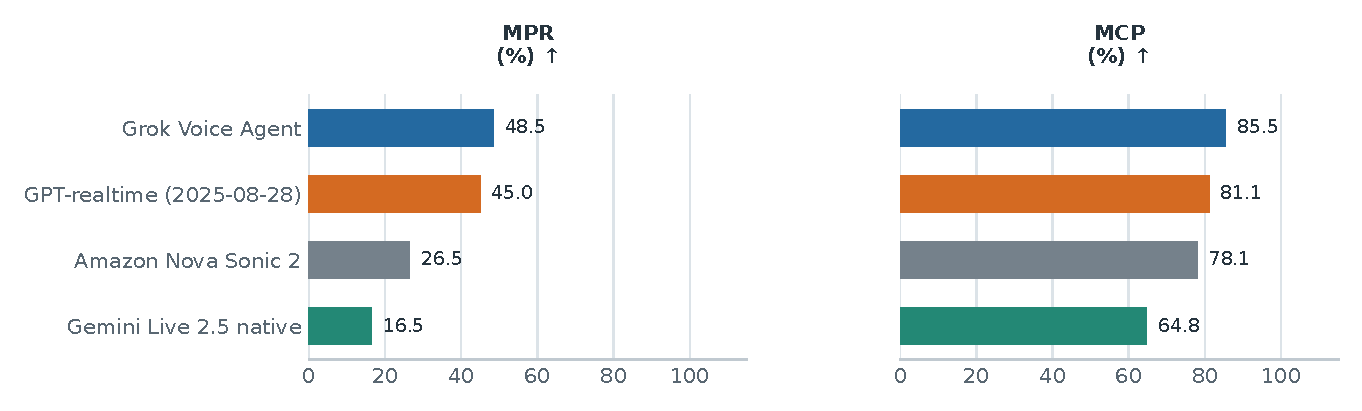
\includegraphics[width=\linewidth]{figures/performance/echochain.pdf}
\caption{EchoChain: closed voice references. Units and directions are labeled per panel. Exact values and additional context references are in the adjacent table.}
\label{fig:performance-echochain}
\end{figure}
% Generated by scripts/build_performance.py; edit research/reported-performance.json.
\begin{table}[H]
\centering\small
\setlength{\tabcolsep}{3pt}
\setlength{\tablewidth}{\dimexpr\linewidth-4\tabcolsep\relax}
\renewcommand{\arraystretch}{1.06}
\caption{EchoChain. Percent; higher is better. Bold: best among the displayed references, not a source-wide or current SoTA. \citep{echochain}}
\label{tab:performance-echo}
\begin{tabular}{@{}>{\raggedright\arraybackslash}p{0.32\tablewidth}>{\centering\arraybackslash}p{0.340000\tablewidth}>{\centering\arraybackslash}p{0.340000\tablewidth}@{}}
\toprule
\textbf{Model / configuration} & \textbf{MPR} & \textbf{MCP} \\
\midrule
Grok Voice Agent & \textbf{48.5} & \textbf{85.5} \\
GPT-realtime-2025-08-28 & 45.0 & 81.1 \\
Amazon Nova Sonic 2 & 26.5 & 78.1 \\
Gemini Live 2.5 native audio & 16.5 & 64.8 \\
\bottomrule
\end{tabular}
\end{table}

{\small\textbf{Reading this profile (review interpretation).} Passing many individual criteria does not guarantee complete conversation success. Even the strongest reported voice reference passes fewer than half of conversations.}
\paragraph{Text controls, not voice competitors.}
GPT-5 (reasoning, text): 85\% (Text task pass@1). Text control, not a realtime voice result. \citep{tauvoice}\par
Gemini 3.1 Pro (explicit, transcript): 94.70 / 90.39 / 95.37\% (Response presence / Conditional answer / Silence preservation). Table 17 reference run; not acoustic, not a speech-model upper bound. \citep{mpe}\par
Gemini 3.1 Pro (implicit, transcript): 30.40 / 79.11 / 99.34\% (Response presence / Conditional answer / Silence preservation). No fresh-onset or stopping score; speaker-attributed transcript is supplied. \citep{mpe}\par

\clearpage
\section{Synchronization as causal consistency across clocks}
\label{sec:clocks}
\paragraph{Listening synchronization: availability is not incorporation.}
For speaker $s$ and input frame $j$, let $c_{s,j}$ be capture time, $a_{s,j}$ arrival time at the runtime, and $i_{s,j}$ the time its encoded evidence has been incorporated into reasoning state. On a synchronized coordinator clock, causal processing requires $i_{s,j}\geq a_{s,j}\geq c_{s,j}$; encoder lookahead and compute backlog contribute different delays. Define an evidence watermark by
\begin{equation}
\label{eq:watermark}
w_s(t)=\max\{j:\max_{r\leq j}i_{s,r}\leq t\},\qquad E_s(t)=t-c_{s,w_s(t)}.
\end{equation}
Here $w_s$ is the latest fully incorporated prefix, and $E_s$ its evidence age. An empty stream has an explicit ``no evidence yet'' state, not a fabricated age; dropped input must be logged, not silently counted as incorporated. Token count or audio merely received by the network is not a substitute for this watermark. Silence/VAD frames should advance the capture timeline too. Clock offsets must be calibrated if capture happens on a separate device.

\paragraph{Speaking synchronization: generation is not commitment.}
For output segment $k$, distinguish generation time $g_k$ from playback time $p_k\geq g_k$. Private reasoning steps occur on a third, compute-dependent timeline; backend completion is another event stream. Maintain the observed audible frontier $A(t)$ separately from queued text, codec and waveform output. A queued segment may be tagged with an evidence watermark and hypothesis/dependency version. A changed version triggers \emph{revalidation}, not automatic deletion of every segment: some earlier claims remain correct. Unplayed output can be withheld or regenerated; heard output requires explicit repair and cannot be rolled back.

\begin{figure}[htbp]
\centering
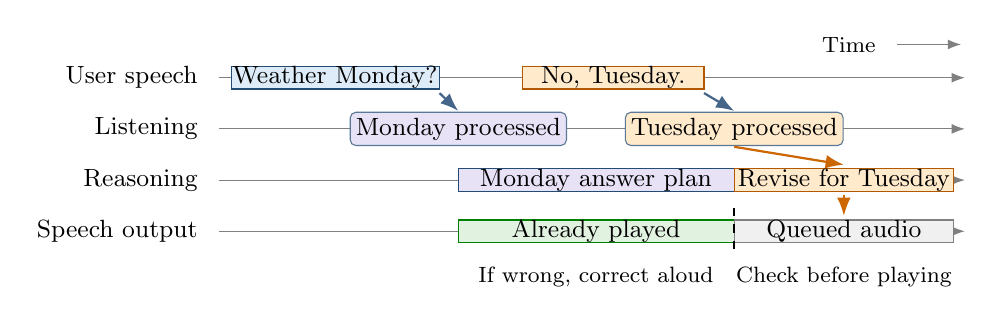
\begin{tikzpicture}[arch,x=0.96cm,y=0.65cm]
\foreach \y/\label in {3/User speech,2/Listening,1/Reasoning,0/Speech output} {
  \node[anchor=east] at (2.13,\y) {\label};
  \draw[->,gray] (2.28,\y)--(12.15,\y);
}
\draw[fill=audiocolor,draw=reportblue] (2.45,2.78) rectangle (5.20,3.22);
\node at (3.82,3) {Weather Monday?};
\draw[fill=mindcolor,draw=orange!70!black] (6.30,2.78) rectangle (8.70,3.22);
\node at (7.50,3) {No, Tuesday.};
\node[model,minimum height=0.40cm,inner sep=2pt] at (5.45,2) {Monday processed};
\node[mind,minimum height=0.40cm,inner sep=2pt] at (9.10,2) {Tuesday processed};
\draw[flow] (5.20,2.7)--(5.45,2.35);
\draw[flow] (8.70,2.7)--(9.10,2.35);
\draw[fill=statecolor,draw=reportblue] (5.45,0.78) rectangle (9.10,1.22);
\node at (7.27,1) {Monday answer plan};
\draw[fill=mindcolor,draw=orange!70!black] (9.10,0.78) rectangle (12.00,1.22);
\node at (10.55,1) {Revise for Tuesday};
\draw[->,orange!80!black,thick] (9.10,1.65)--(10.55,1.30);
\draw[fill=voicecolor,draw=green!50!black] (5.45,-0.22) rectangle (9.10,0.22);
\node at (7.27,0) {Already played};
\draw[fill=gray!12,draw=gray] (9.10,-0.22) rectangle (12.00,0.22);
\node at (10.55,0) {Queued audio};
\draw[->,orange!80!black,thick] (10.55,0.70)--(10.55,0.30);
\draw[dashed,thick] (9.10,-0.35)--(9.10,0.50);
\node[note,anchor=north,text width=3.4cm] at (7.27,-0.50) {If wrong, correct aloud};
\node[note,anchor=north,text width=2.9cm] at (10.55,-0.50) {Check before playing};
\node[note,anchor=east] at (11.10,3.65) {Time};
\draw[->,gray] (11.25,3.65)--(12.10,3.65);
\end{tikzpicture}

\caption{Illustrative Monday-to-Tuesday correction, not an experimental result. User speech may enter as audio tokens or acoustic features. Once the correction is processed, revise the answer plan and check queued audio before playback. Wrong claims already played need an audible correction; they cannot be taken back.}
\label{fig:clocks}
\end{figure}

\paragraph{A testable output-admission policy.}
Let $Q(t)$ be the unplayed audio queue and $d_k$ each segment's remaining audible duration. A candidate policy imposes
\begin{equation}
\label{eq:admission}
H(t)=\sum_{k\in Q(t)} d_k\leq H_{\max}(t),\qquad
\operatorname{admit}(k,t)\Rightarrow\operatorname{valid}(\operatorname{deps}(k),\operatorname{state}(t)).
\end{equation}
The cap may adapt to correction risk or available compute; unrendered text lead requires an estimated speech duration, not a universal tokens-to-seconds conversion. Dependency validity is a proposed observable/controller target, \emph{not} an oracle guarantee that a claim is semantically true. A small in-flight hardware buffer creates residual stop latency that must be measured. Figure~\ref{fig:clocks} makes these separate commitment points explicit. This framing extends rather than replaces existing acoustic clocks and cancellation mechanisms.

\section{Five major research questions}
\label{sec:questions}
All questions are hypotheses to test, not claims of established novelty. They map to the proposal's sufficiency, revision, speaker ownership and useful-response objectives. The first three separate private thought, audible commitment and fresh listening; the fourth studies their scheduler; the fifth extends revision to delegated work.

\researchquestion{RQ1}{Think while listening: sufficient for what, and at what risk?}
\textbf{Question.} When is a speech prefix sufficient to begin useful reasoning, and when should its hypothesis remain provisional? \textbf{Hypothesis.} A causal prefix trigger calibrated for correction risk improves the correct-answer/latency frontier over end-of-turn and fixed-prefix triggers. Begin private work early but gate task-specific spoken claims separately. \textbf{Minimal test.} Construct 200 matched late-constraint questions with two suffixes sharing exactly the same prefix. Hold input watermarks and decoding budgets fixed; compare end-of-turn, fixed-prefix and calibrated triggers, including held-out speaking rates. Measure correct useful audible response time, final accuracy, premature claims, calibration and unnecessary revisions. \textbf{Prior-work boundary.} Early explicit reasoning and latent listening-time computation already exist \citep{thinklisten,flair}. The potential contribution is correction-risk calibration under causal delayed evidence, not ``thinking before the user finishes.'' An oracle suffix-aware trigger is an upper bound only, never a deployable baseline.

\researchquestion{RQ2}{Think while speaking: how much uncommitted lead is safe?}
\textbf{Question.} How far can reasoning and synthesis run ahead of playback before a late correction makes the spoken answer stale? \textbf{Hypothesis.} Evidence-tagged output and a bounded playback lead reduce stale audible claims at matched compute and answer quality. \textbf{Minimal test.} Inject an otherwise identical correction before generation, during synthesis, while audio is queued, and after it becomes audible. Compare unrestricted lead, a fixed-duration cap, and dependency-aware admission; revalidate only unplayed output and explicitly repair heard errors. Measure stale audible duration, useful-response time, underruns, repetitions and repair success. \textbf{Prior-work boundary.} Mind-Paced Speaking and StepAudio 3 already separate formulation from articulation; AdaptDuplex already bounds text lead \citep{mindpaced,step3,adapt}. EchoChain already tests interrupted reasoning \citep{echochain}. The candidate contribution is a measured causal playback commitment policy, not concurrent reasoning itself or fast filler speech.

\researchquestion{RQ3}{Listen while speaking: whose evidence changes whose state?}
\textbf{Question.} Can fresh input update the appropriate speaker/task hypothesis during speaking without treating a backchannel or side conversation as a correction? \textbf{Hypothesis.} Per-speaker evidence watermarks and selective dependency invalidation improve correction accuracy without increasing false interruption or unsolicited responses. \textbf{Minimal test.} Match relevant corrections against backchannels and other-directed utterances. Compare one global reasoning state with speaker/task-owned versions under generation contention. First use oracle speaker/addressee labels, then predicted labels, to isolate attribution from reasoning errors. Measure evidence age, correction accuracy, silence preservation, false interruption and task success. \textbf{Prior-work boundary.} Duplex-MPE evaluates addressee behavior, and synchronization probes reveal timing signals \citep{mpe,synchrony}. Our proposed extension couples speaker attribution to state revision and listening freshness; it is not a new diarization or turn-taking problem in isolation.

\researchquestion{RQ4}{Synchronize the clocks under variable rates and load}
\textbf{Question.} Which temporal interface keeps listening, reasoning and speaking consistent when speech rate, inference speed and network delay vary independently? \textbf{Hypothesis.} A controller observing evidence age and queued-audio duration reduces missed deadlines and stale claims at matched task accuracy. \textbf{Minimal test.} Replay identical short dialogues under controlled rate, jitter and compute contention. Compare fixed scheduling with a two- or three-level adaptive quantum, preserving feature extraction and model capabilities; use 80 ms or 1 s reference interfaces only where the runtime supports them. Report p50/p95 ingestion and useful-response delays, underruns, missed deadlines, quality and GPU-seconds. \textbf{Prior-work boundary.} SyncLLM, Moshi, MiniCPM-o, DuplexSLA and AdaptDuplex already represent or adapt time \citep{syncllm,moshi,minicpm,duplexsla,adapt}. The open test is causal robustness under heterogeneous clocks, with physical timing in addition to virtual-time task results \citep{tauvoice}. Faster hardware must not be credited as a modeling gain.

\researchquestion{RQ5}{Revise while delegating: which result is still admissible?}
\textbf{Question.} When a correction arrives between backend launch, result return and audible delivery, what should be canceled, reused or withheld? \textbf{Hypothesis.} Speaker/task-dependent checks at both result admission and playback improve corrected task success beyond cancellation and stale-result suppression alone. \textbf{Minimal test.} Use read-only or simulated tools with 0.5, 2 and 5 s backend delays; inject corrections at launch, inflight, return and pre-playback stages. Compare blind result injection, an explicit cancellation/stale-suppression baseline, and joint result/output revalidation. Measure stale-result use, task success, wasted work, unnecessary cancellation and repair latency. \textbf{Prior-work boundary.} Realtime-Venus and Context Spanning provide delegation/injection designs; AdaptDuplex rejects canceled/stale results, and DuplexOmni stops/resets background thinking \citep{venus,contextspan,adapt,duplexomni}. VoiceChat's tool-execution barge-in restriction is a distinct baseline condition, not an interruption-capable control \citep{voicechat}. The potential extension is joint speaker-owned and audible-commitment consistency. Real irreversible tool actions require a \emph{separate} action-commit protocol; cancellation cannot undo an executed side effect.

\section{A controlled first study and reporting protocol}
\label{sec:protocol}
Start with a released, instrumentable 7--9B runtime (Moshi, MiniCPM-o or the Venus harness, according to the hooks the study needs), not foundation-scale reproduction. Build a 200--500-case causal-prefix pilot with small paired variations: late relevant constraint versus irrelevant/backchannel input; correction before versus after an audible claim; and, where relevant, same versus different speaker/addressee. Use a simulated read-only backend for deterministic timing. Establish access and licensing before introducing natural recordings; document the synthetic-to-natural transition rather than silently mixing conditions. No GPU jobs are launched by this report.

Log timestamps for capture, arrival and incorporation, together with source/hypothesis versions, generated text/codec/audio boundaries, actual playback, cancellation/admission events, and task outcomes. Define the \emph{first useful correct audible response} as the earliest task-specific claim that is correct given the evidence incorporated at that time; report latency relative to both the gold sufficient-prefix endpoint and actual sufficient-evidence incorporation. Score correctness separately against evidence physically available to the runtime, so an agent cannot obtain a good freshness score merely by delaying ingestion. Distinguish first token, first audio/filler, private-reasoning onset, useful answer, tool request, task completion and interruption stop time. Include stale audible seconds and whether an incorrect heard claim was successfully repaired.

Use paired task-level comparisons and confidence intervals, not independent reruns with different prompts or audio. Hold feature lookahead, available evidence, task split, model/harness revision, decode budget, backend delay and judge configuration fixed. Report accuracy--latency--commitment trade-offs, rather than a single weighted score that hides premature errors. Natural corpus splits must be by source session and speaker where appropriate; machine-generated labels need manual auditing. Oracle speaker labels, future-aware sufficiency and backend gold answers are diagnostic upper bounds only. Virtual-clock simulation and physical-clock playback are separate experimental conditions.

\section{Limitations and intended contribution}
\label{sec:limits}
The shortlists are deliberately focused, not exhaustive. Recent preprints and artifact statuses can change; open inference does not imply reproducible training. Reported scales and licenses come from resource documentation, not a full provenance audit. No published scores are independently reproduced here, and none of the proposed hypotheses has been validated. The five research questions are unranked; eight concrete candidate implementations and their risks/estimated pilot costs are supplied in the accompanying research notes, not presented as selected winners. Each novelty claim needs further search before a paper submission.

The central proposal update is to treat \emph{listening freshness} and \emph{speaking commitment} as separate, measurable synchronization obligations. Timing-aware interfaces already exist. A meaningful next contribution would show when correctly attributed new evidence can revise ongoing reasoning, pending work and unplayed output without either stale audible claims or unnecessary disruption---and characterize the regimes in which that approach fails.

\begingroup
\footnotesize
\setlength{\bibsep}{1pt}
\bibliography{references}
\bibliographystyle{iclr2026_conference}
\endgroup
\end{document}
